% User guide
The Robot Operating System (ROS) is a software framework for developing robotic systems in a metaoperating system environment. The primary goal of ROS is to support code reuse in robotics research and development.

ROS is a collection of tools, libraries, and conventions that aim to simplify the task of creating complex and robust robot behavior across a wide variety of robotic platforms.
ROS provides the services you would expect from an operating system, including hardware abstraction, low-level device control, implementation of commonly-used functionality, messagepassing between processes, and package management.
It also provides tools and libraries for obtaining, building, writing, and running code across multiple computers. 

ROS is comprised of a number of independent nodes, each of which communicates with the other nodes using a publish /subscribe messaging model "we will explain this soon". 
ROS was originally developed in 2007 at the Stanford Artificial Intelligence Laboratory and development continued at Willow Garage. It is managed by the Open Source Robotics Foundation.\\


\textbf{Ready} to get started with ROS ? You’ve come to the right place. Here you will find our collection of step-by-step tutorials.\\


\textbf{First}, you must know that ROS is a framework which only runs on Unix-based platforms" We used Ubuntu". 
We used ROS Kinetic Kame distribution, which is available for Ubuntu Xenial(16.04 LTS), among other platform options.


 \section{Prerequisites to start with ROS}
 	Before getting started with ROS and trying code, the following prerequisites should be met:\\
 
 	\textbf{First}, We have to use Ubuntu as the operating system for installing ROS.
  	Its prefer to stick on to the L.T.S version of Ubuntu, that is, \url{www.releases.ubuntu.com/16.04.2/} Ubuntu 16.04.2 LTS (Xenial Xerus).\\
  	Hint, select an image which is suitable for you, then burn it into removable storage with any software like rufus, and the installation will done using the GUI guide.
  	If you don't use ubuntu operating system or any distribution of unix before, Don't worry, we will explain the concepts at the ubuntu operating system section. 
  	Now, Install the full desktop installation of ROS. The following link gives you the installation instruction of the L.T.S ROS distribution: \url{http://wiki.ros.org/kinetic/Installation/Ubuntu}. 
  	Hint, Just follow the installation instructions which is copying the commands from the website and paste it in the command line window on your PC.
 \section{General Concepts}
 	The basic building blocks of Robot Operating System "ROS software framework are Packages. ROS works as a group of programs everyone is called Node. Every Package contains a collection of Nodes. ROS starts with the ROS Master node. The Master node allows all other ROS pieces of software (Nodes) to find and talk to each other. Every Node communicate with each other through Messages.
 	\begin{itemize}
 		\item \textbf{Packages}:\\
 		 The ROS packages are the most basic unit of the ROS software. It contains the ROS runtime process (nodes), libraries, configuration files, and so on, which are organized together as a single unit. Packages are the atomic build item and release item in the ROS software. 
 		 \item \textbf{Package manifest}: The package manifest file is inside a package that contains information about the package, author, license, dependencies, compilation flags, and so on. The package.xml file inside the ROS package is the manifest file of that package.
 	\end{itemize}
 	
	\subsection{Structure of a typical ROS package}
	package.xml: This is the package manifest file of this package.\\
    CMakeLists.txt: This is the CMake build file of this package.\\
    msg: This folder contains custom message definitions.\\
    srv: This folder contains the service definitions. \\
    include/package\_name: This folder consists of headers and libraries that we need to use inside the package. \\
    scripts: This folder keeps executable Python scripts. \\
    src: This folder stores the C++ source codes.\\
    We need to know some commands to create, modify, and work with the ROS packages.
    Here are some of the commands used to work with ROS packages:
    \begin{itemize}
    	\item \textbf{catkin\_create\_pkg}: This command is used to create a new package.
    	\item \textbf{rospack}: This command is used to get information about the package in the file system.
    	\item \textbf{catkin\_make}: This command is used to build the packages in the workspace.
    	\item \textbf{rosdep}: This command will install the system dependencies required for this package.
    \end{itemize}

	\subsection{Messages (.msg)}
	
	The ROS messages are a type of information that is sent from one ROS process to the other, we can define a custom message inside the msg folder inside a package (my\_package/msg/ MyMessageType.msg), the extension of the message file is .msg, ROS nodes can publish data having a particular type and communicate with each other using messages.
	The types of data are described using a simplified message description language, also called ROS messages, these datatype descriptions can be used to generate source code for the appropriate message type in different target languages.
	
	 Messages are simply a data structure containing the typed field, which can hold a set of data and that can be sent to another node. There are standard primitive types (integer, floating point, Boolean, and so on) and these are supported by ROS messages. We can also build our own message types using these standard types.
	 
	 Here are some parameters used along with rosmsg:
	 \begin{itemize}
	 	\item rosmsg show [message]: This shows the message description. 
	 	\item rosmsg list: This lists all messages. 
	 	\item rosmsg package [package\_name]: This lists messages in a package.
	 	\item rosmsg packages [package\_1] [package\_2]: This lists packages that contain messages.
	 \end{itemize}
 	\subsection{Services (.srv)}
 	The ROS service is a kind of request/reply interaction between processes (Nodes), one node can send a request and wait until it gets a response from the other.
 	The request/response communication is also using the ROS message description. 
 	The reply and request data types can be defined inside the srv folder inside the package (my\_package/srv/MyServiceType.srv).
 	
 	In some robot applications, a publish/subscribe model will not be enough if it needs a request/response interaction. The publish/subscribe model is a kind of one-way transport system and when we work with a distributed system, we might need a request/response kind of interaction.
 	
 	ROS Services are used in these case. We can define a service definition that contains two parts; one is for requests and the other is for responses. 
 	Using ROS Services, we can write a server node and client node. The server node provides the service under a name, and when the client node sends a request message to this server, it will respond and send the result to the client. The client might need to wait until the server responds. The ROS service interaction is like a remote procedure call.
 	
 	The following explain how to use the rosservice tool to get information about the running services:
 	
 	\begin{itemize}
 		\item rosservice call /service args: This tool will call the service using the given arguments.
 		\item rosservice find service\_type: This command will find services in the given service type.
 		\item rosservice info /services: This will print information about the given service.
 		\item rosservice list: This command will list the active services running on the system.
 		\item rosservice type /service: This command will print the service type of a given service.
 		\item rosservice uri /service: This tool will print the service ROSRPC URI.
 	\end{itemize}
 
 	\subsection{Topics}
 	Each message in ROS is transported using named buses called topics. When a node sends a message through a topic, then we can say the node is publishing a topic. When a node receives a message through a topic, then we can say that the node is subscribing to a topic. The publishing node and subscribing node are not aware of each other's existence. We can even subscribe a topic that might not have any publisher. In short, the production of information and consumption of it are decoupled. Each topic has a unique name, and any node can access this topic and send data through it as long as they have the right message type.
 	
 	The ROS topic tool can be used to get information about ROS topics. Here is the syntax of this command:
 	
 	\begin{itemize}
 		\item rostopic bw /topic: This command will display the bandwidth used by the given topic.
 		\item rostopic echo /topic: This command will print the content of the given topic. 
 		\item rostopic find /message\_type: This command will find topics using the given message type. 
 		\item rostopic hz /topic: This command will display the publishing rate of the given topic. 
 		\item rostopic info /topic: This command will print information about an active topic. 
 		\item rostopic list: This command will list all active topics in the ROS system. 
 		\item rostopic pub /topic message\_type args: This command can be used to publish a value to a topic with a message type.
 		\item rostopic type /topic: This will display the message type of the given topic.
 	\end{itemize}
 
 	\subsection{Nodes}
 	Nodes are the process that perform computation. Each ROS node is written using ROS client libraries such as roscpp and rospy. In a robot, there will be many nodes to perform different kinds of tasks. Using the ROS communication methods, it can communicate with each other and exchange data. One of the aims of ROS nodes is to build simple processes rather than a large process with all functionality. Being a simple structure, ROS nodes are easy to debug too.
 	
 	One node can communicate with other nodes using ROS Topics, Services, and Parameters. A robot might contain many nodes, for example, one node processes camera images, one node handles serial data from the robot, and so on.
 	
 	Using nodes can make the system fault tolerant. Even if a node crashes, an entire robot system can still work. Nodes also reduce the complexity and increase debug-ability compared to monolithic codes because each node is handling only a single function.
 	
 	All running nodes should have a name assigned to identify them from the rest of the system. For example, /camera\_node could be a name of a node that is broadcasting camera
 	images.
 	
 	\begin{figure}[h]		
 		\centering
 		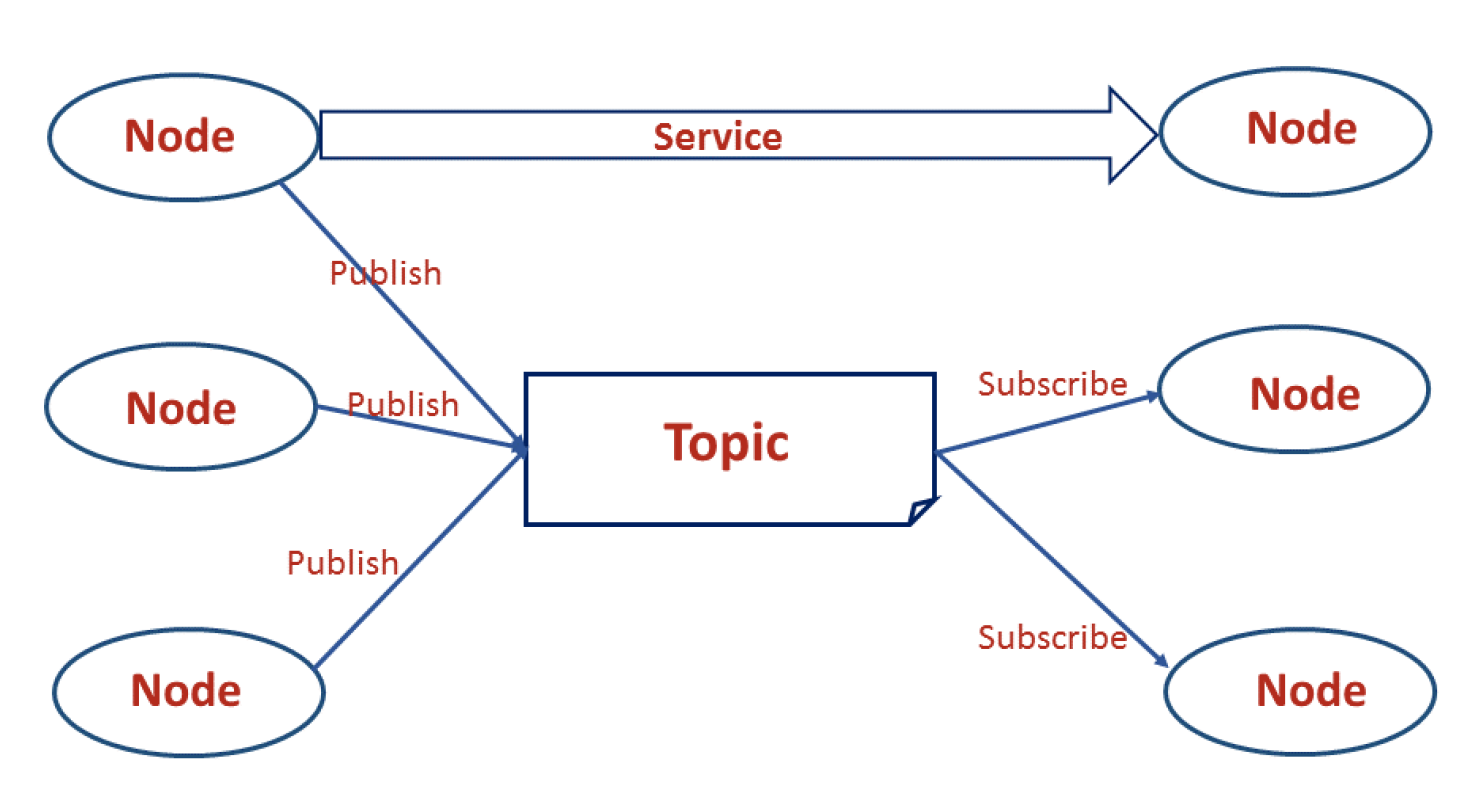
\includegraphics[width =.8\textwidth]{Nodes}
 		\caption{Communicating nodes.}
 		\label{Fig:Node}
 	\end{figure}
 
	There is a rosbash tool to introspect ROS nodes.
	The rosnode command can be used to get information about a ROS node. Here are the usages of rosnode:
	\begin{itemize}
		\item rosnode info [node\_name]: This will print the information about the node.
		\item rosnode kill [node\_name]: This will kill a running node.
		\item rosnode list: This will list the running nodes.
		\item rosnode ping: This will check the connectivity of a node.
		\item rosnode machine [machine\_name]: This will list the nodes running on a particular machine or a list of machines.
		\item rosnode cleanup: This will purge the registration of unreachable nodes.
	\end{itemize}
	 
	 \subsection{Master}
	 The ROS Master provides name registration and lookup to the rest of the nodes. Nodes will not be able to find each other, exchange messages, or invoke services without a ROS Master. In a distributed system, we should run the master on one computer, and other remote nodes can find each other by communicating with this master.
	 
	 When any node starts in the ROS system, it will start looking for ROS Master and register the name of the node in it. So ROS Master has the details of all nodes currently running on the ROS system. When any details of the nodes change, it will generate a call-back and update with the latest details. These node details are useful for connecting with each node.
	 
	 When a node starts publishing a topic, the node will give the details of the topic such as name and data type to ROS Master. ROS Master will check whether any other nodes are subscribed to the same topic. If any nodes are subscribed to the same topic, ROS Master will share the node details of the publisher to the subscriber node.
	 
	 After getting the node details, these two nodes will interconnect using the TCPROS protocol, which is based on TCP/IP sockets. After connecting to the two nodes, ROS Master has no role in controlling them. We might be able to stop either the publisher node or the subscriber node according to our wish. If we stop any nodes, it will check with ROS Master once again.The following is a command to start ROS Master and the ROS parameter server : \$ roscore
	 
	 \begin{figure}[h]		
	 	\centering
	 	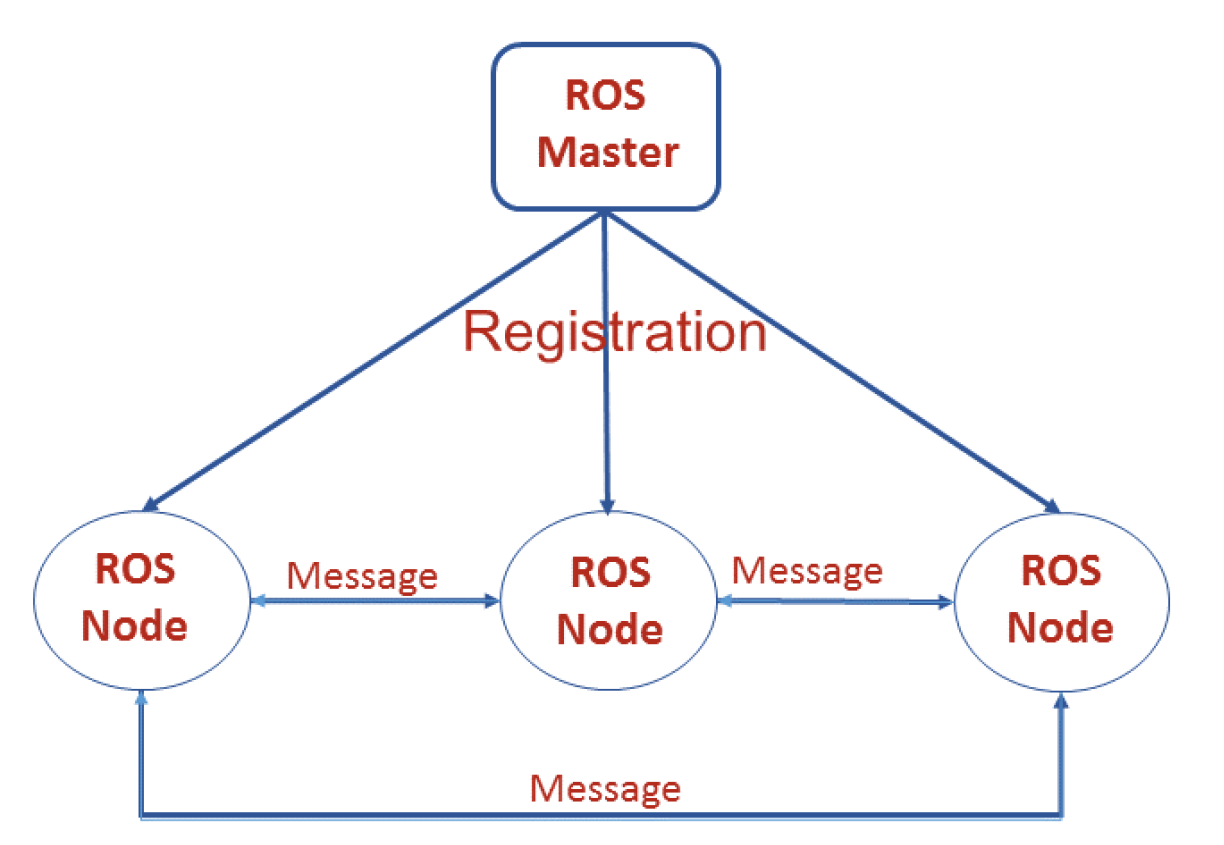
\includegraphics[width =.8\textwidth]{Master}
	 	\caption{Registration and lookup the nodes.}
	 	\label{Fig:Master}
	 \end{figure}
 
\section{Creating a ROS Workspace \& Package}
 The ROS packages are the basic unit of the ROS system. We can create the ROS package, build it and release it to the public. The current distribution of ROS we are using is Kinetic Kame. We are using the catkin build system to build ROS packages.
 
 A build system is responsible for generating 'targets'(executable/libraries) from a raw source code that can be used by an end user. In older distributions, such as Electric and Fuerte, rosbuild was the build system. Because of the various flaws of rosbuild, catkin came into existence, which is basically based on CMake (Cross Platform Make).
 
 \textbf{CMake} has lot of advantages such as porting the package into other operating system, such as Windows. If an OS supports CMake and Python, catkin based packages can be easily ported into it. The first requirement in creating ROS packages is to create a ROS catkin workspace.
 
 Build a workspace folder in the home directory and create a src folder inside the workspace folder:
 \begin{itemize}
 	\item \lstinline|$ mkdir ~/catkin_ws/src|
 	Switch to the source folder. The packages are created inside this package:
 	\item \lstinline|$ cd ~/catkin_ws/src|
 	Initialize a new catkin workspace:
 	\item \lstinline|$ catkin_init_workspace|
	We can build the workspace even if there are no packages. We can use the following command to switch to the workspace folder:
 	\item \lstinline|$ cd ~/catkin_ws|
 	The catkin\_make command will build the following workspace:
 	\item \lstinline|$ catkin_make|
 \end{itemize}

 After building the empty workspace, we should set the environment of the current workspace to be visible by the ROS system.
 This process is called overlaying a workspace. We should add the package environment using the following command:
 \begin{itemize}
 	\item \lstinline|$ echo "source ~/catkin_ws/devel/setup.bash" >> ~/.bashrc |
 	\item \lstinline|$ source ~/.bashrc|
 \end{itemize}
 This command will source a bash script called setup.bash inside the devel workspace folder. To set the environment in all bash sessions, we need to add a source command in the .bashrc file, which will source this script whenever a bash session starts.
 
 This is the link of the procedure \url{www..wiki.ros.org/catkin/Tutorials/create\_a\_workspace}.
 
 \begin{enumerate}
 	\item After setting the catkin workspace, we can create our own package that has sample nodes to demonstrate the working of ROS topics, messages, services, and actionlib.
 	\item The catkin\_create\_pkg command is used to create a ROS package in which we are going to create demos of various ROS concepts.
 	\item Switch to the catkin workspace src folder and create the package using the following command: 
     \begin{lstlisting}[language=terCmd]
    $ catkin\_create\_pkg [package\_name] [dependency1] [dependency2]
     \end{lstlisting}
     Example:
      \begin{lstlisting}[language=terCmd]
 $ catkin\_create\_pkg zaghexa\_pkg roscpp std\_msgs actionlib actionlib\_msgs
     \end{lstlisting}

 	\item After creating this package, build the package without adding any nodes using the catkin\_make command. This command must be executed from the catkin workspace path. The following command shows you how to build our empty ROS package: 
       \begin{lstlisting}[language=terCmd]
     $ ~/catkin_ws
     $ catkin_make
     \end{lstlisting}
     

 	\item After a successful build, we can start adding nodes to the src folder of this package.
 \end{enumerate}
 Hint, The dependencies in the packages are:
 \begin{itemize}
 	\item \textbf{roscpp}: This is the C++ implementation of ROS. It is a ROS client library which provides APIs to C++ developers to make ROS nodes with ROS topics, services, parameters, and so on. We are including this dependency because we are going to write a ROS C++ node. Any ROS package which uses the C++ node must add this dependency.
 	\item \textbf{std\_msgs}: This package contains basic ROS primitive data types such as integer, float, string, array, and so on. We can directly use these data types in our nodes without defining a new ROS message.
 	\item \textbf{actionlib}: The actionlib meta-package provides interfaces to create preemptable tasks in ROS nodes. We are creating actionlib based nodes in this package. So we should include this package to build the ROS nodes.
 	\item \textbf{actionlib\_msgs}: This package contains standard message definitions needed to interact with the action server and action client.	
 \end{itemize}

\section{Creating ROS nodes}

\subsection{Publisher}
 The first node we are going to discuss is publisher.cpp.
 This node will publish an integer value on a topic called /numbers. Here is the detailed explanation of the preceding code:
 
\begin{lstlisting}[language=C++]
 #include "ros/ros.h"
 #include "std\_msgs/Int32.h"
 #include <iostream>
 
 void main()
 {
    ros::init(argc, argv,"publisher");
    ros::NodeHandle node\_obj;
    ros::Publisher number\_publisher = node\_obj.advertise<std\_msgs::Int32>("/numbers",10);
    ros::Rate loop\_rate(10);
    while (ros::ok()) {
        std\_msgs::Int32 msg;
        msg.data = number\_count;
        ROS\_INFO("%d",msg.data);
        number\_publisher.publish(msg);
        ros::spinOnce();
        loop\_rate.sleep();
    }
 }
 \end{lstlisting}
 
 The \textit{ros/ros.h} is the main header of ROS. If we want to use the \textit{roscpp} client APIs in our code, we should include this header. 
 The \textit{std\_msgs/Int32.h} is the standard message definition of integer datatype.
 Here, we are sending an integer value through a topic. So we should need a message type for handling the integer data. \textit{std\_msgs} contains standard message definition of primitive datatypes. \textit{std\_msgs/Int32.h} contains integer message definition: \textit{ros::init(argc, argv,"publisher");} This code will initialize a ROS node with a name. It should be noted that the ROS node should be unique. This line is mandatory for all ROS C++ nodes: \textit{ros::NodeHandle node\_obj;}
 
 This will create a \textit{Nodehandleobject}, which is used to communicate with the ROS system:
 \textit{ ros::Publisher number\_publisher = node\_obj.advertise<std\_msgs::Int32>("/numbers",10);} 
 This will create a topic publisher and name the topic /numbers with a message type \textit{std\_msgs::Int32}. The second argument is the buffer size. It indicates that how many messages need to be put in a buffer before sending. It should be set to high if the data sending rate is high: \textit{ros::Rate loop\_rate(10);} This is used to set the frequency of sending data:\textit{ while (ros::ok()) } This is an infinite while loop, and it quits when we press Ctrl+C. The\textit{ ros::ok()} function returns zero when there is an interrupt; this can terminate this while loop:
 \textit{std\_msgs::Int32 msg;} 
 \textit{msg.data = number\_count;} 
 The first line creates an integer ROS message and the second line assigns an integer value to the message.
 Here, data is the field name of the msg object:\textit{ ROS\_INFO("\%d",msg.data);} This will print the message data. This line is used to log the ROS information: \textit{number\_publisher.publish(msg);}
 This will publish the message to the topics /numbers:\textit{ ros::spinOnce();} 
 This command will read and update all ROS topics, the node will not publish without a spin() or spinOnce() function.
 \textit{ loop\_rate.sleep();}
 This line will provide the necessary delay to achieve a frequency of 10Hz.

 
 \subsection{Subscriber}
 
  After discussing the publisher node, we can discuss the subscriber node, which is subscriber .cpp. Copy the code to a new file or use the existing file.
  \begin{lstlisting}[language=C++]
#include "ros/ros.h"
#include "std_msgs/Int32.h"
#include <iostream>

/*This is a callback function that will execute whenever a data comes to the /numbers topic. Whenever a data reaches this topic, the function will call and extract the value and print it to the console.*/
void number_callback(const std_msgs::Int32::ConstPtr & msg) 
{ ROS_INFO("Recieved [%d]",msg->data); }

void main()
{
    ros::init(argc, argv,"subscriber");
    ros::NodeHandle node_obj;
    
    /*This is the subscriber and here, we are giving the topic name needed to subscribe, buffer size, and callback function:
        > we are subscribing /numbers topic
        > we have already seen the callback function above*/
    ros::Subscriber number_subscriber = node_obj.subscribe("/numbers",10,number_callback);
    
    /* This is an infinite loop in which the node will stay: 
    > This code will invoke the callbacks whenever a data reaches the topic. 
    > The node will quit only when we press the Ctrl+C key */
    ros::spin();
}

  \end{lstlisting}
  This is the header needed for the subscribers.

%  \lstinline|void number_callback(const std_msgs::Int32::ConstPtr\& msg){ ROS_INFO("Recieved [\%d]",msg->data); } |\\
%  This is a callback function that will execute whenever a data comes to the /numbers topic.
%  Whenever a data reaches this topic, the function will call and extract the value and print it on the console.
%  
%\lstinline|ros::Subscriber number_subscriber = node_obj.subscribe("/numbers",10,number_callback);|\\
%This is the subscriber and here, we are giving the topic name needed to subscribe, buffer size, and the callback function. 

%  We are subscribing /numbers topic and we have already seen the callback function in the preceding section: \lstinline|ros::spin();|
%  This is an infinite loop in which the node will wait in this step. This code will fasten the callbacks whenever a data reaches the topic. The node will quit only when we press the Ctrl+C key.

 \section{Control Servo motor using Joystick}
 
 \begin{enumerate}
 	\item First change to the source space directory of the catkin workspace\\
      \lstinline|$ cd ~/catkin_ws/src|
     
     
 	\item Now use the catkin\_create\_pkg script to create a new package called ‘servo1’ which depends on \verb|std_msgs, roscpp,| and \verb|rospy|:\\
     \lstinline|$ catkin_create_pkg servo1 std_msgs rospy roscpp|
     
 	\item Now you need to build the packages in the catkin workspace:\\
    \lstinline|$ catkin\_make|
     
 	\item To add the workspace to your ROS environment you need to source the generated setup file:\\
         \lstinline|$ ~/catkin_ws/devel/setup.bash|
         
 	\item In your /home you will find the work space folder : catkin\_ws inside you will find the created package which called : servo1 inside it the source folder which will include the codes \& CMAKElists.txt which includes all the dependencies \& the required components.
     
 	\item In folder source /src: create a new document let's call it 'servotry.cpp' and copy the code here inside this file \& save it then close.
     
 	\item In CMakeLists.txt we will add the dependencies which is needed to run the code \& for building it: please delete all comments to make the view clearer and make the code the same as this:
 	\begin{lstlisting}[language=XML]
 	cmake_minimum_required (VERSION 2.8.3) 
 	project(servo1)
 	find_package(catkin REQUIRED COMPONENTS
 	joy
 	roscpp
 	rospy
 	std_msgs
 	geometry_msgs
 	sensor_msgs )
 	catkin_package()
 	include_directories(
 	${catkin_INCLUDE_DIRS}
 	)
 	add_executable(servotry src/servotry.cpp)
 	target_link_libraries(servotry ${catkin_LIBRARIES})
 	add_dependencies(servotry servo1_generate_messages_cpp)
 \end{lstlisting}
     \item Save the CMakeLists.txt then close it.
 	
     \item Important: Check that the created package: 'servo1' folder is in the path : /catkin\_ws/src
 	if not move the folder servo1 from '/catkin\_ws' into '/catkin\_ws/src'
 	
     \item In "servo1" folder create new folder call it "launch" \& inside "launch" create new document and call it "servorun.launch" then open using text editor and insert the following code:\\
     \begin{lstlisting}[language=XML]
     <launch>
     <!-- joy node -->
     <node respawn="true" pkg="joy"
     type="joy_node" name="joy_node" >
     <param name="dev" type="string" value="/dev/input/js0" />
     <param name="moda" value="0.1" />
     </node>
     <!-- Axes -->
     <param name="axis_linear" value="1" type="int"/>
     <param name="axis_angular" value="0" type="int"/>
     <param name="scale_linear" value="2" type="double"/>
     <param name="scale_angular" value="2" type="double"/>
     <node pkg="jost" type="ser" name="servo_joy"/>
     </launch>
     \end{lstlisting}
 	As we created the code we need to build it, go to your package directory : 
     \begin{lstlisting}[language=terCmd]
$ cd catkin_ws
$ source devel/setup.bash
$ catkin_make
     \end{lstlisting}

     \item Now Arduino
 	Arduino role here is to subscribe to the joystick 'the publisher' to take the joystick readings and map it to the servo that's connected to the Arduino so that it gives the servo the signal to move to the specified location using given degree.
 	\item If you don't have Arduino IDE please check this tutorial: \url{www.wiki.ros.org/rosserial_arduino/Tutorials/Arduino%20IDE%20Setup}
 	for step by step installation once you complete the install open the Arduino IDE and jump to next step.
 	\item Write Arduino code:
 		\begin{lstlisting}[language=C++]
 	#if (ARDUINO >= 100)
 	#include <Arduino.h>
 	#else
 	#include <WProgram.h>
 	#endif
 	#include <Servo.h>
 	#include <ros.h>
 	#include <std_msgs/UInt16.h>
 	ros::NodeHandle nh;
 	Servo servo;
 	void servo_cb( const std_msgs::UInt16& cmd_msg){
 	if(cmd_msg.data==2)
 	{
 	servo.write(180);
 	}
 	else if(cmd_msg.data==65534)
 	{
 	servo.write(0);
 	}
 	else
 	{servo.write(90);}
 	}
 	ros::Subscriber<std_msgs::UInt16> sub("servo", servo_cb);
 	void setup(){
 	
 	nh.initNode();
 	nh.subscribe(sub);
 	
 	servo.attach(9); //attach it to pin 9
 	}
 	void loop(){
 	nh.spinOnce();
 	delay(1);
 	}
 	\end{lstlisting}
 	\item Save then upload to your Arduino, don't forget to choose your board type \& the serial port.
 	
 	Note: if you COULDN'T UPLOAD to Arduino \& the upload stopped with the message: \emph{"couldn't open port"}, do the following:
     \begin{itemize}
         \item from Arduino tools menu see the port address it will be like "/dev/ttyUSB0" and REMEMBER IT.
         \item Then open new terminal \& type: \\
         \lstinline|$ sudo usermod -a -G dialout <TYPE YOUR USERNAME>|
         
         \item Write your password then:\\
         \lstinline|$ sudo chmod a+rw /dev/<TYPE YOUR PORT ADDRESS>|
         
         Example:
         \begin{lstlisting}[language=terCmd]
 $ sudo usermod -a -G dialout khaled
 $ sudo chmod a+rw /dev/ttyUSB0
         \end{lstlisting}
     \end{itemize}

     \item After uploading the code, Open new terminal to start. don't forget to \textbf{connect the joystick}.
 	
     \item To initialize the master, type: \lstinline|$ roscore|
 	\item Open new tab, start the communication between ROS \& Arduino using serial Type :\\
 	\lstinline|$ rosrun rosserial_python serial_node.py <YOUR PORT ADDRESS>| 

     Example: \lstinline|$ rosrun rosserial_python serial_node.py /dev/ttyUSB0|

    \item Wait to start.
     
 	\item Finally open new tab go to \verb|catkin_ws|, then type:
     \begin{lstlisting}[language=terCmd]
$ cd catkin_ws
$ source devel/setup.bash
$ roslaunch servo1 servorun.launch
     \end{lstlisting}
 \end{enumerate}


\section{Setting ROS on Raspberry Pi 3B}

Raspberry Pi3 is single board computers which have low form factor with a size of a credit card. This single board computer can be installed in robots and we can install ROS on it.
One of the popular single board computers is Raspberry Pi. The Raspberry Pi boards are manufactured by Raspberry Pi Foundation which is based in the UK. The latest model of Raspberry Pi is Raspberry Pi 3B. The official website of Raspberry Pi is \url{www.raspberrypi.org} .

\subsection{Environment}
We can install Ubuntu and Android on Raspberry Pi. There are also unofficial distributions of Linux such as Debian mini, Kali Linux, Arch Linux, and Fedora, and also support libraries such as ROS, OpenCV, PCL, and so on .
For getting ROS on Raspberry Pi , we can either install a fresh Ubuntu and install ROS manually or install Ubuntu which is inbuilt with ROS, OpenCV, and PCL.
Installing ROS from the source code and packages will take several hours. 
The official guide of installing ROS on Raspberry Pi 2 into their official OS is available at \url{wiki.ros.org/indigo/Installation/UbuntuARM} .
The Raspberry Pi 3 official OS images are given at \url{www.raspberrypi.org/downloads/} .The official OS supported by Raspberry Pi foundation are Raspbian and Ubuntu. There are unofficial images based on this OS which has ROS pre-installed on them.

\subsection{How to install an OS image to Raspberry Pi}

We installed a fresh Ubuntu and install ROS manually. 

\textbf{Installation in Windows}

In Windows, there is a tool called Win32 disk image which is designed specifically for Raspberry Pi . You can download the tool from \url{www.raspberry-projects.com/pi/pi-operating-systems/win32diskimager} , run Win32 Disk Imager with the Administrator privilege.

Select the downloaded image  "Ubuntu mate" download it from \url{ubuntu-mate.org/raspberry-pi/} , select the memory card drive, and write the image to the drive.

\begin{figure}[h]		
	\centering
	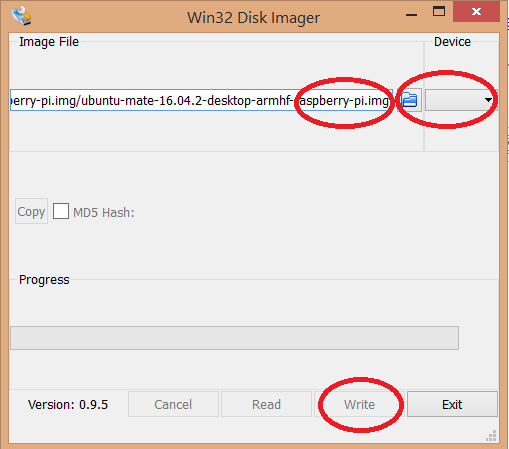
\includegraphics[width =.8\textwidth]{win32}
	\caption{Registration and lookup the nodes.}
	\label{Fig:Win32}
\end{figure}

After completing this wizard, we can put the micro SD card in Raspberry Pi and boot up the OS "Ubuntu mate". Then, you can install ROS from the source code \url{wiki.ros.org/kinetic/Installation/Ubuntu}, now, you have Raspberry Pi support ROS.

\subsection{Connecting to Raspberry Pi from a PC}

We can work with Raspberry Pi  by connecting to the HDMI display port and connect the keyboard and mouse to the USB like a normal PC.\\
This is the simplest way of working with Raspberry Pi.

In most of the projects, the boards will be placed on the robot, so we can't connect the display and the keyboards to it. There are several methods for connecting these boards to the PC. 
It will be good if we can share the Internet to these boards too. The following methods can share the Internet to these boards, and at the same time, we can remotely connect via SSH protocol:

\begin{itemize}
	\item \textbf{Remote connection using Wi-Fi router and Wi-Fi dongle through SSH:}
\end{itemize}
In this method, we need a Wi-Fi router with Internet connectivity. 
Both the PC and board will connect to the same network, so each will have an IP address and can communicate using that address.

\begin{itemize}
	\item \textbf{Direct connection using an Ethernet hotspot:}
\end{itemize}

We can share the Internet connection and communicate using SSH via Dnsmasq, a free software DNS forwarder and DHCP server using low system resources. Using this tool, we can tether the Wi-Fi Internet connection of the laptop to the Ethernet and we can connect the board to the Ethernet port of the PC. This kind of communication can be used for robots which are static in operation.

The first method is very easy to configure; it's like connecting two PCs on the same network. 
The second method is a direct connection of board to laptop through the Ethernet. This method can be used when the robot is not moving.
In this method, the board and the laptop can communicate via SSH at the same time and it can share 
Internet access too. We are using this method in this chapter for working with ROS.

\subsection{Making Raspberry connect automatically to our network at start up }
First of all as we always like to work remotely without need to stuck beside raspberry, but the problem is that raspberry by default on startup the wifi adapter detects the networks available in the surrounding area. so to avoid conflict between the networks we will assign it to work with our network and search for it. 
if it found, prioritize it and connect to it.
First go to : /etc/network/interfaces
then add:
\begin{lstlisting}[language=XML]
auto wlan0
	iface wlan0 inet dhcp 
	wpa-ssid {ssid}
	wpa-psk  {password}
\end{lstlisting}
Then run this in terminal:
\begin{lstlisting}[language=XML]
sudo dhclient wlan0
\end{lstlisting}
\textbf{Note}:

\begin{itemize}
\item SSID : is the network name you want it to auto connect\\
\item This configuration is done once on fresh installed system. 

\end{itemize}
\clearpage
\section{Connect raspberry pi 3 and arduino with serial usb cable}


\begin{figure}[h]
	\centering
	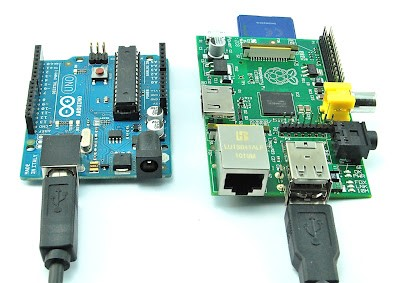
\includegraphics[width=8.47cm,height=5.99cm]{figures/s12.jpg}
\end{figure}


\textbf{\begin{center}
		Using USB Cable Between Raspberry Pi and Arduino
\end{center}}

There are many ways of connecting the Raspberry Pi and Arduino, such as 
using the GPIO and Serial pins and using I2C. But this could be one of the easiest way to get them talking, because hardware  that required is minimal: all you will need is a micro USB cable that comes with the Arduino. 
First of all, make sure you have installed pySerial, which 
gives you the ability to read from and write to the serial port with Python Programming language. 

\subsection{Arduino Talking to Raspberry Pi via USB cable}
We will send 'Hi ZagHexa' from the Arduino to the Raspberry Pi every 2 seconds. 
Here is the Arduino source code.
\begin{lstlisting}[language=XML]

void setup(){
Serial.begin(9600);}

void loop(){
Serial.println("Hi ZagHexa");
delay(2000);}
\end{lstlisting}

Run Python 2 on Raspberry Pi. You will find this from the menu under 
Programming, you should use Python 2 not 3.

Type the following:
\begin{lstlisting}[language=XML]
import serial
ser = serial.Serial('/dev/ttyACM0', 9600)
\end{lstlisting}
The first argument - /dev/ttyACM0 is the name for the USB interface used. To find out the port name, we need to run this command in terminal without Arduino plugged in:
\begin{lstlisting}[language=XML]
ls /dev/tty*
\end{lstlisting}
Now plug in your Arduio and run the command again. If a new name appears, then this is the name of your port.

The second argument - 9600 is the baud rate and should match with what 
you set in the Arduino program.

Now lets start a loop listening for messages from the Arduino.
\begin{lstlisting}[language=XML]
while 1 :
ser.readline()
\end{lstlisting}
You will need two hit enter twice after you type the second line. 
Messages 'Hi ZagHexa' should now start to appear every 2 seconds. You can press Ctrl + C to stop (interrupt) the Python program.

\subsection{Raspberry Pi Sending Data To Arduino}
In this example, Raspberry Pi will be sending back a single number/character and Arduino will turn on and off the LED on Pin 12 so many times.
\begin{lstlisting}[language=XML]
const int ledPin = 12;

void setup(){
pinMode(ledPin, OUTPUT);
Serial.begin(9600);}

void loop(){
if (Serial.available()){
	light(Serial.read() - '0');}
	delay(500);}
	
void light(int n){
	for (int i = 0; i<n; i++) {
		digitalWrite(ledPin, HIGH);
		delay(100);
		digitalWrite(ledPin, LOW);
		delay(100); } 
	}
\end{lstlisting}
On the Raspberry Pi Side, you need to type
\begin{lstlisting}[language=XML]
ser.write('3')
\end{lstlisting}
\textbf{Now you should see the LED on the Arduino light up 3 times.}